\section{Development process}

Most of the work on this excercise was carried out at the computer lab (room 458, IT-Vest, NTNU). The subject staff has equipped the lab with several workstations running Ubuntu 12.04 LTS. Each workstation is connected to an EFM32GG-DK3750 development board via USB. The toolchain necessary for cross-development is also preinstalled on each workstation. The subject staff also provided a project framework, containing amongst other things a Makefile with some convenient rules configured, a complete linkerscript and a header file containing many usefull memory addresses defined as pointer constants.

To facilitate some off-site development and to ease versioning and teamwork, the project was put under version control, see section \ref{other-tools}. The development process itself was very iterative, with a clear goal emerging after having successfully experimented with generating sound.

\subsection{Devices}
The device used in this exercise is the same as in the previous exercise, the EFM32GG-DK3570 produced by Silicon Labs. It has a built in Digital-Analog Converter which is the primary focus of the exercise.

While the DAC is physically connected to the main processing unit, it functions like a peripheral that must be manually activated before it can be used. A standard $3.5mm$ audio jack socket is available, meaning a normal set of headphones or earplugs can be connected to listen to the DAC output.

As in exercise 1 the only source of user input is the 8-button gamepad peripheral connected to the development board's GPIO pins. In this exercise the 8 LEDs on the gamepad are not the primary means of output, but they are still available if needed.

\begin{figure}[h!]
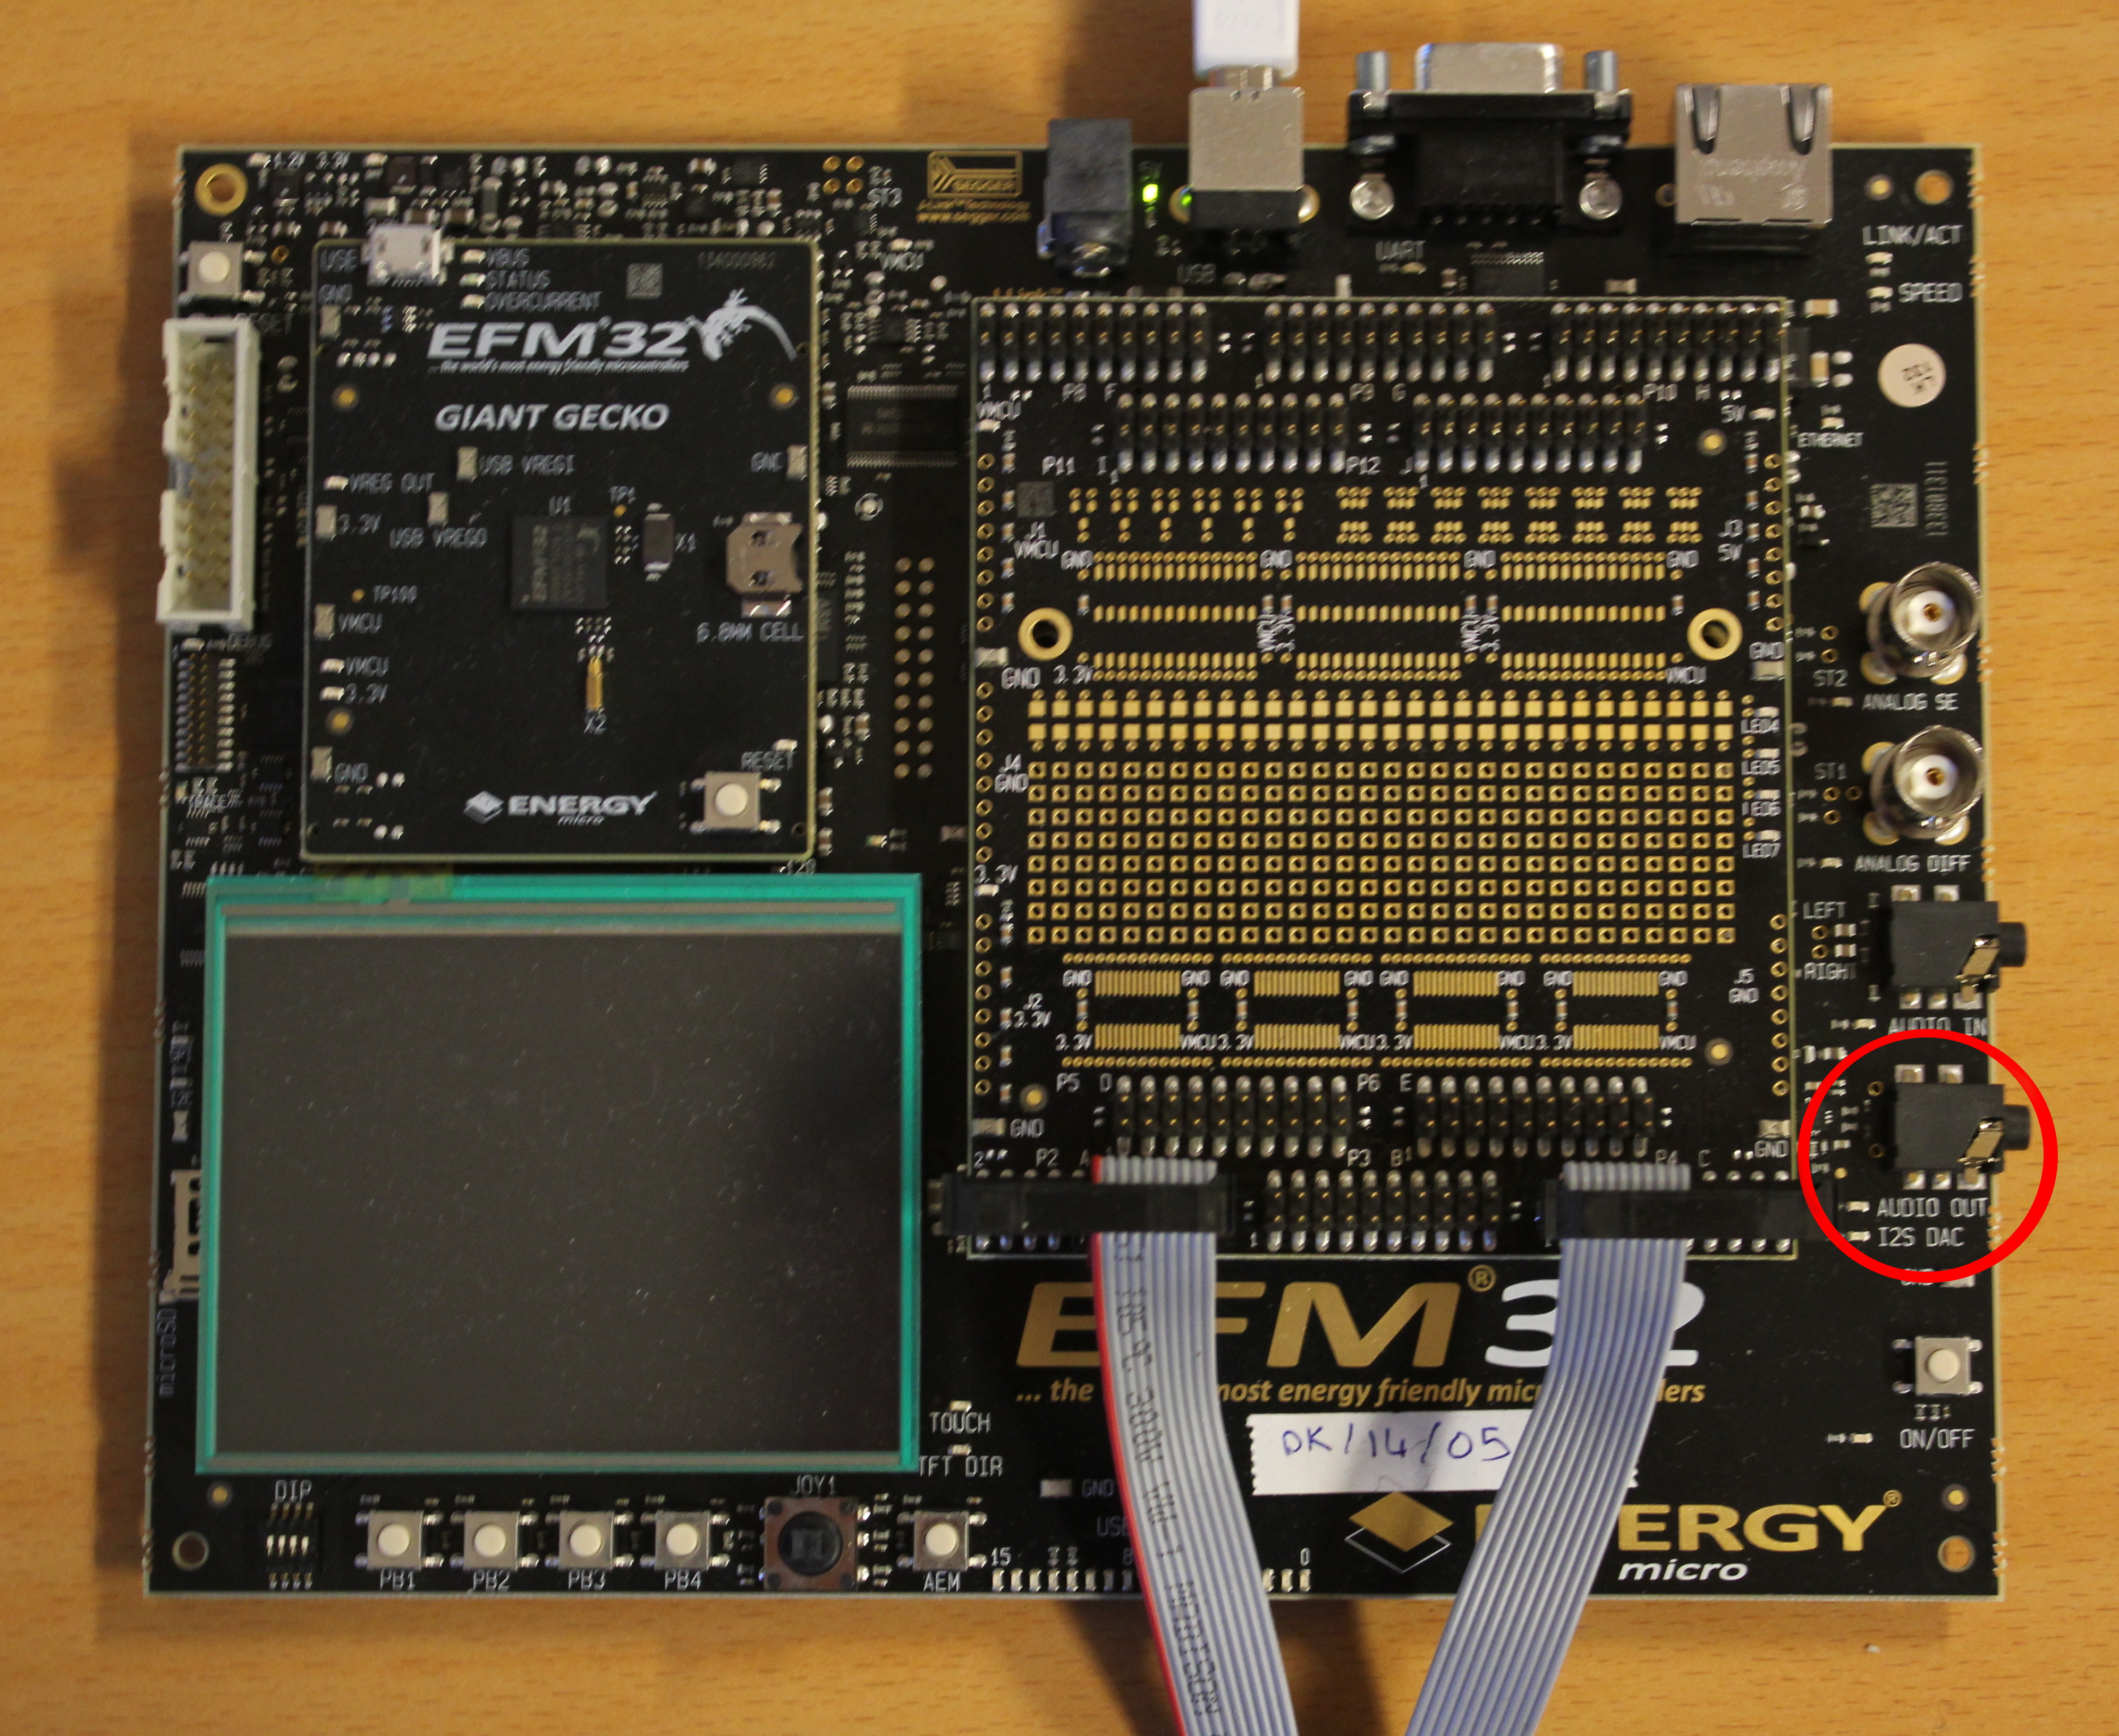
\includegraphics[width=\linewidth]{img/efm32gg.JPG}
\caption{The EFM32GG-DK3570. Highlighted with red is the audio output from the DAC. The gamepad peripheral is connected by the cables emerging on the bottom of the picture.}
\label{fig:efm32gg}
\end{figure}

